% !TeX spellcheck = fr_FR
% !TeX encoding = ISO-8859-1

\section{Rappel par deux bandes}

Ce point semble facile et il l'est. Cependant, pour ramener la 2 dans le
� chapeau �, il demande une grande attention et un bon tour de main. Le
danger vient de la bosse possible de la 2 sur la 1, apr�s deux bandes.

Figure : le point se joue en trois quarts coul�, coup allong� et tr�s
accompagn�, peu ou pas d'effet favorable. La difficult� est la juste
prise de la 2. Prise trop fine, la 2 reste en chemin et ne rentre pas.
Prise trop grosse, la 2 risque de percuter la 1 en deux endroits : voyez
les croisements de trajectoires, particuli�rement le deuxi�me. Une bonne
allonge, donne un peu plus de vitesse � la 1 et permet de ramener sans
bosse.

Le tout est une question de mesure et ... d'entra�nement.

Entra�nement : Comme sur la figure, je conseille de commencer avec la 2
en face de la mouche 3. C'est cet emplacement qui est le plus dangereux
pour la bosse. Une fois cette position acquise, essayez des s�ries avec
la 2 en face de la mouche 2, puis en face de la mouche 1. Vous
constaterez par vous-m�me que plus la 2 est situ�e � haut �, moins
grosse (mais au moins une demi-bille) doit-elle �tre prise pour assurer
le point mais alors, la 2 rentre moins bien ! Pour quand m�me rentrer la
2, il y a deux solutions, soit allonger un peu moins ou jouer plus sec :
Ces derni�res nuances sont difficiles d'application surtout si on ajoute
que pour assurer le retour de la 2, la 1 arrive plus rapidement et
risque de ne pas rester dans le secteur, voire d'�clater la 3. Apr�s ces
brillants essais, on peut encore tenter le coup avec la 2 en face de la
mouche 4. C'est difficile et il ne faut pas descendre au-del�. Il s'agit
d'un vrai coul� sans effet, avec la 1 qui doit absolument passer devant
la 2 avant de toucher la petite bande oppos�e.

Cas particulier : Si la 3 est situ�e � une mouche du coin, le m�me coup
est encore possible avec un l�ger effet contraire haut de bille : plus
facile qu'il n'y para�t.

\begin{figure}[htb]
	\centering
	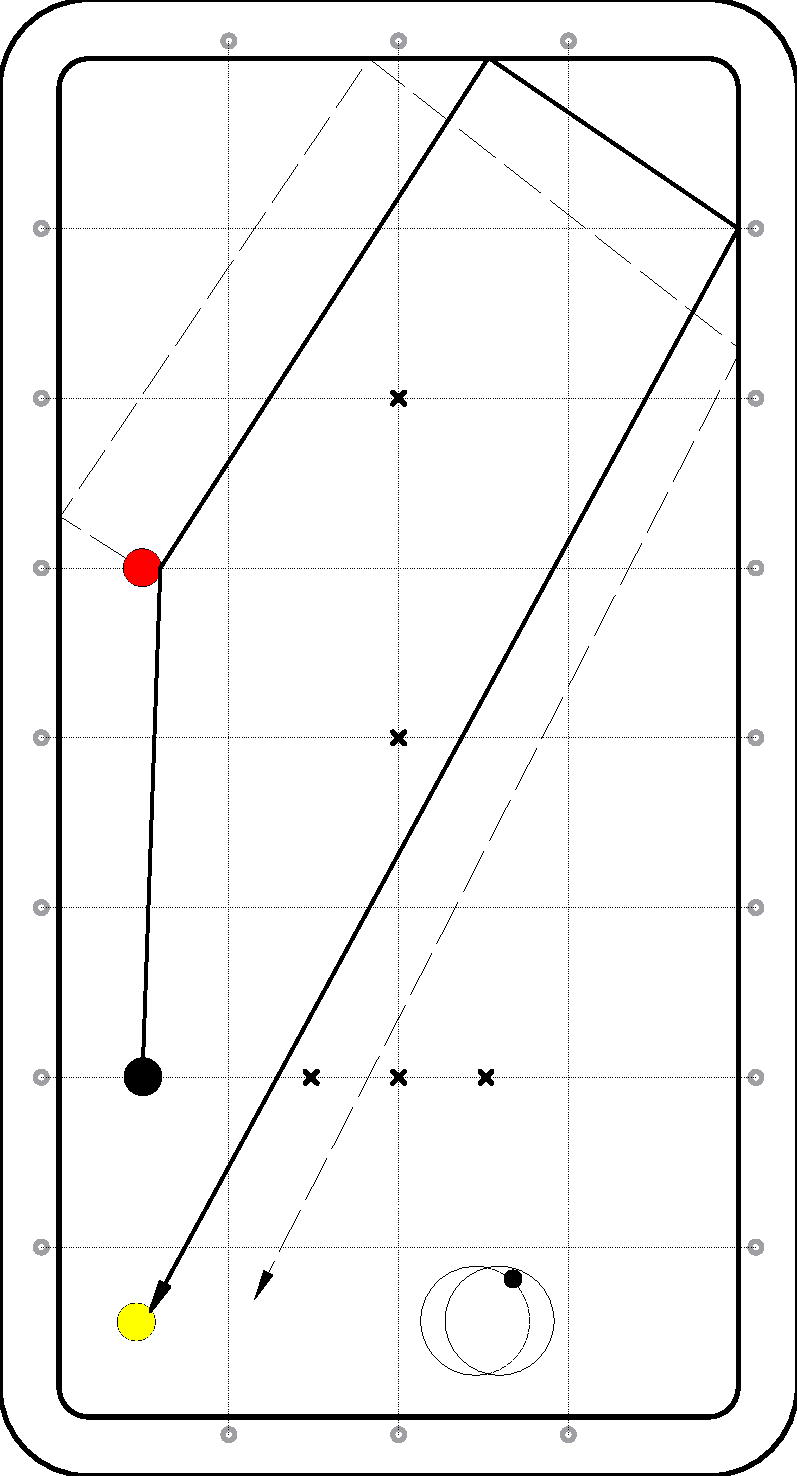
\includegraphics[width=0.85\linewidth]{A/imagesA/A20-01.pdf}
	\caption{Rappel par deux bandes}
	\label{fig:a20-1}
\end{figure}
\clearpage
